%%%%%%%%%%%%%%%%%%% Figure 2 Bathymetry and currents in the Drøbak area %%%%%%%%%%%%%%%
\begin{figure}[t]
 \begin{center}
  \begin{pspicture}(0,0)(15,8.5)
% Include graphs
   \rput[bl](0,0){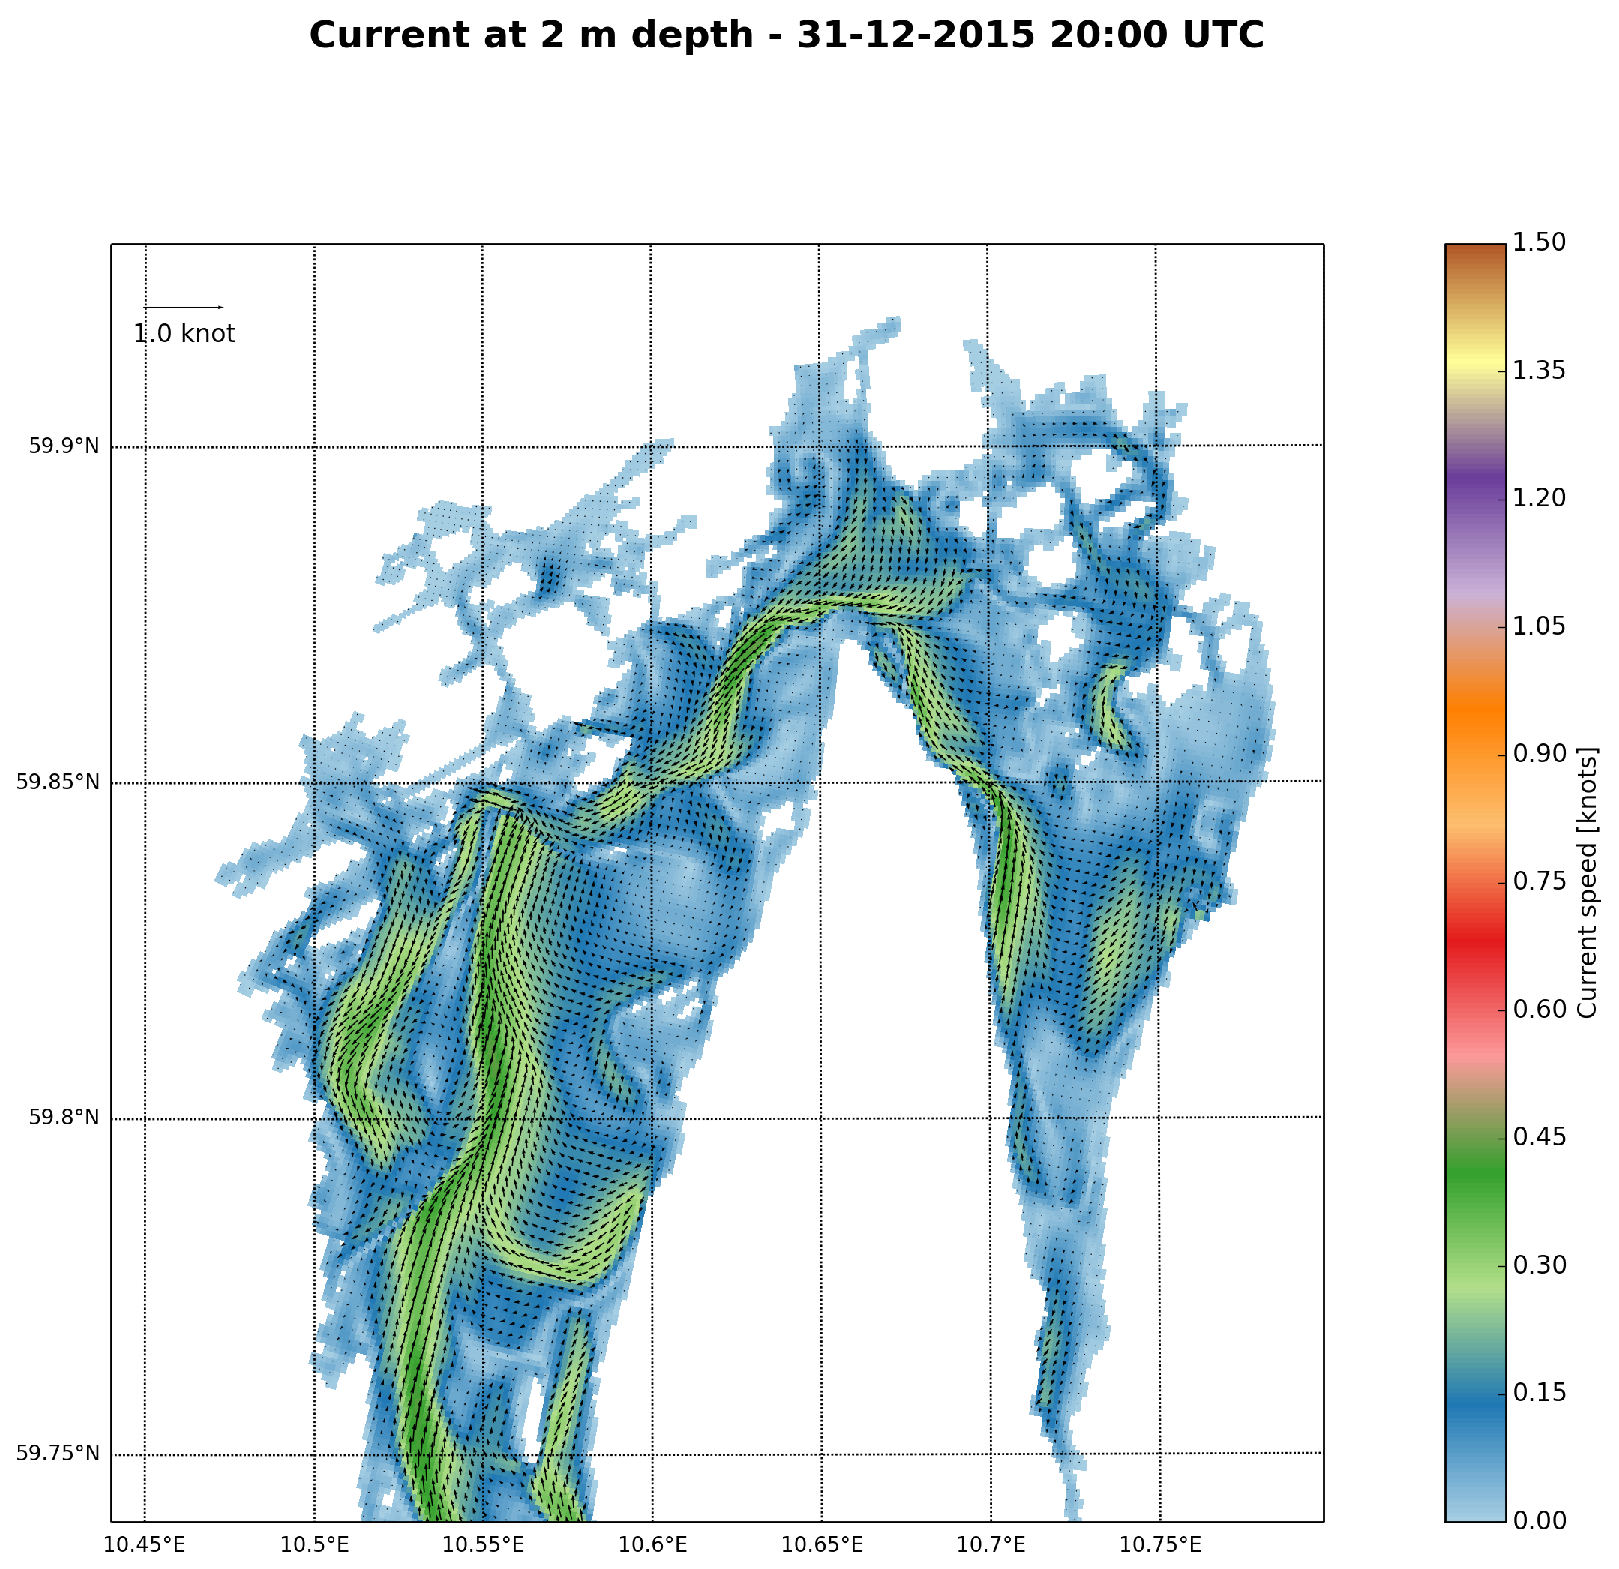
\includegraphics[height=8.5cm]{indre__56_current}}
   \rput[bl](7.5,0){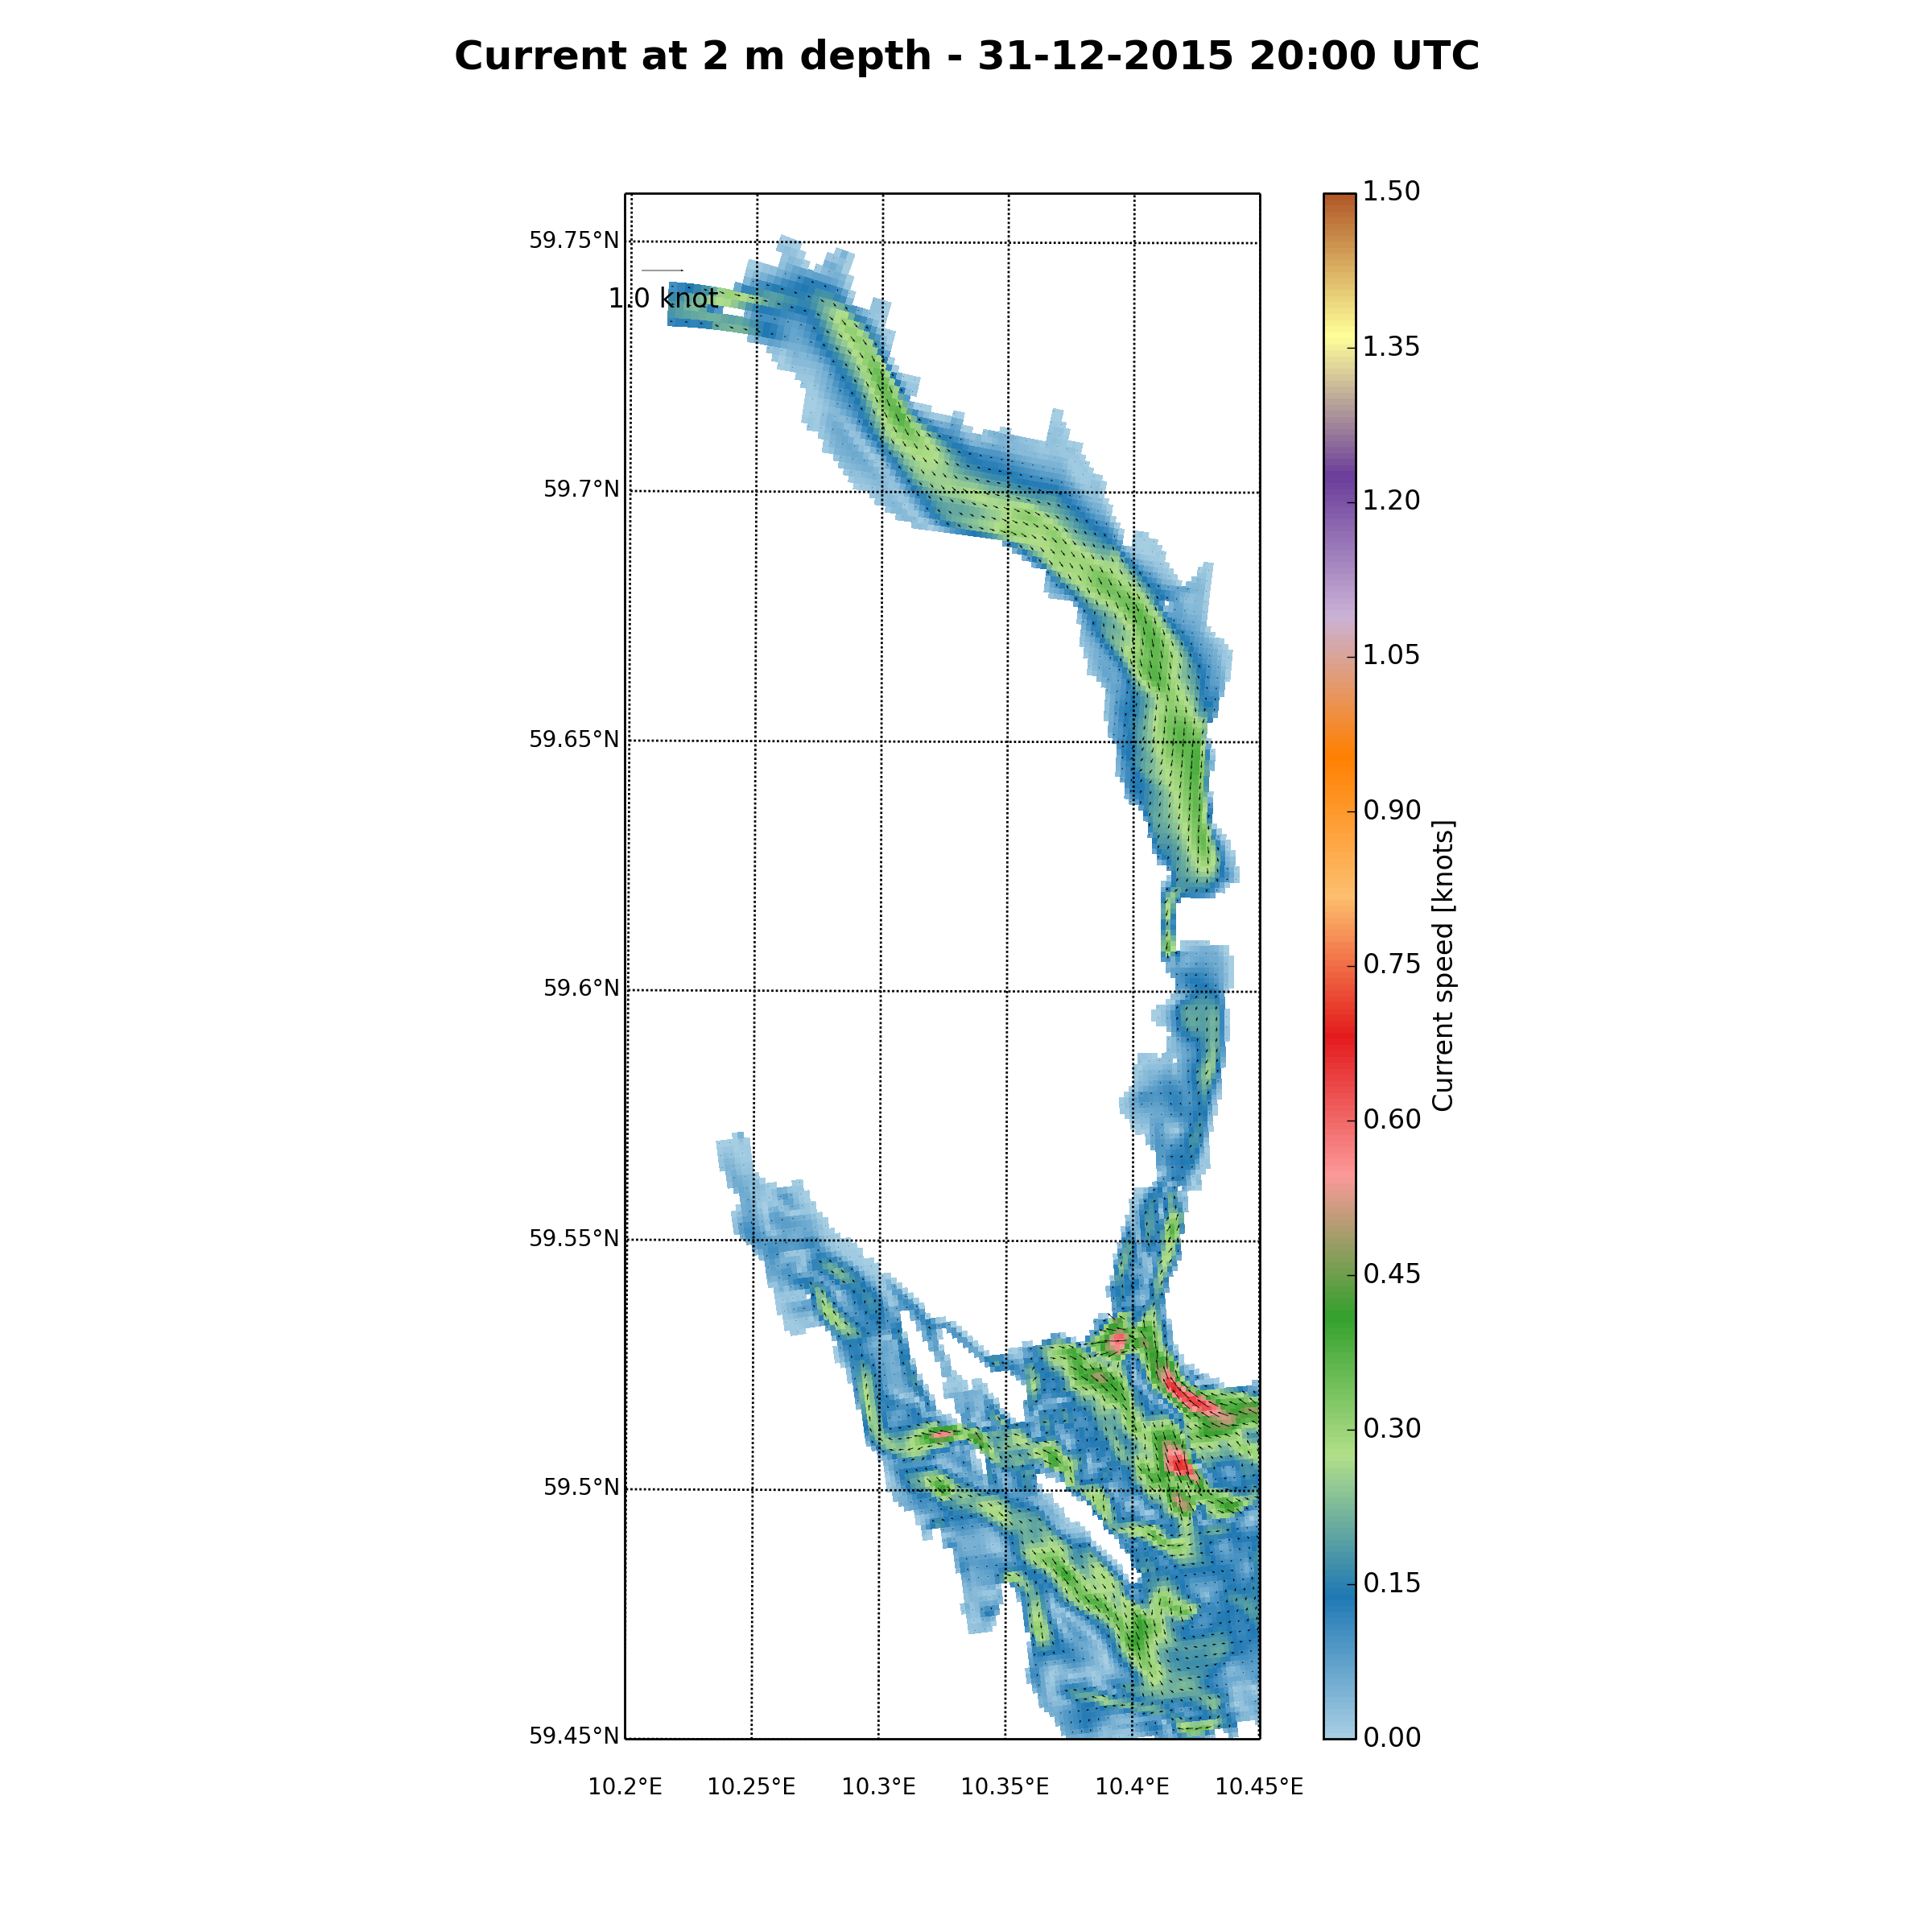
\includegraphics[height=8.5cm]{drammen1__56_current}}
   \rput[br](15,0){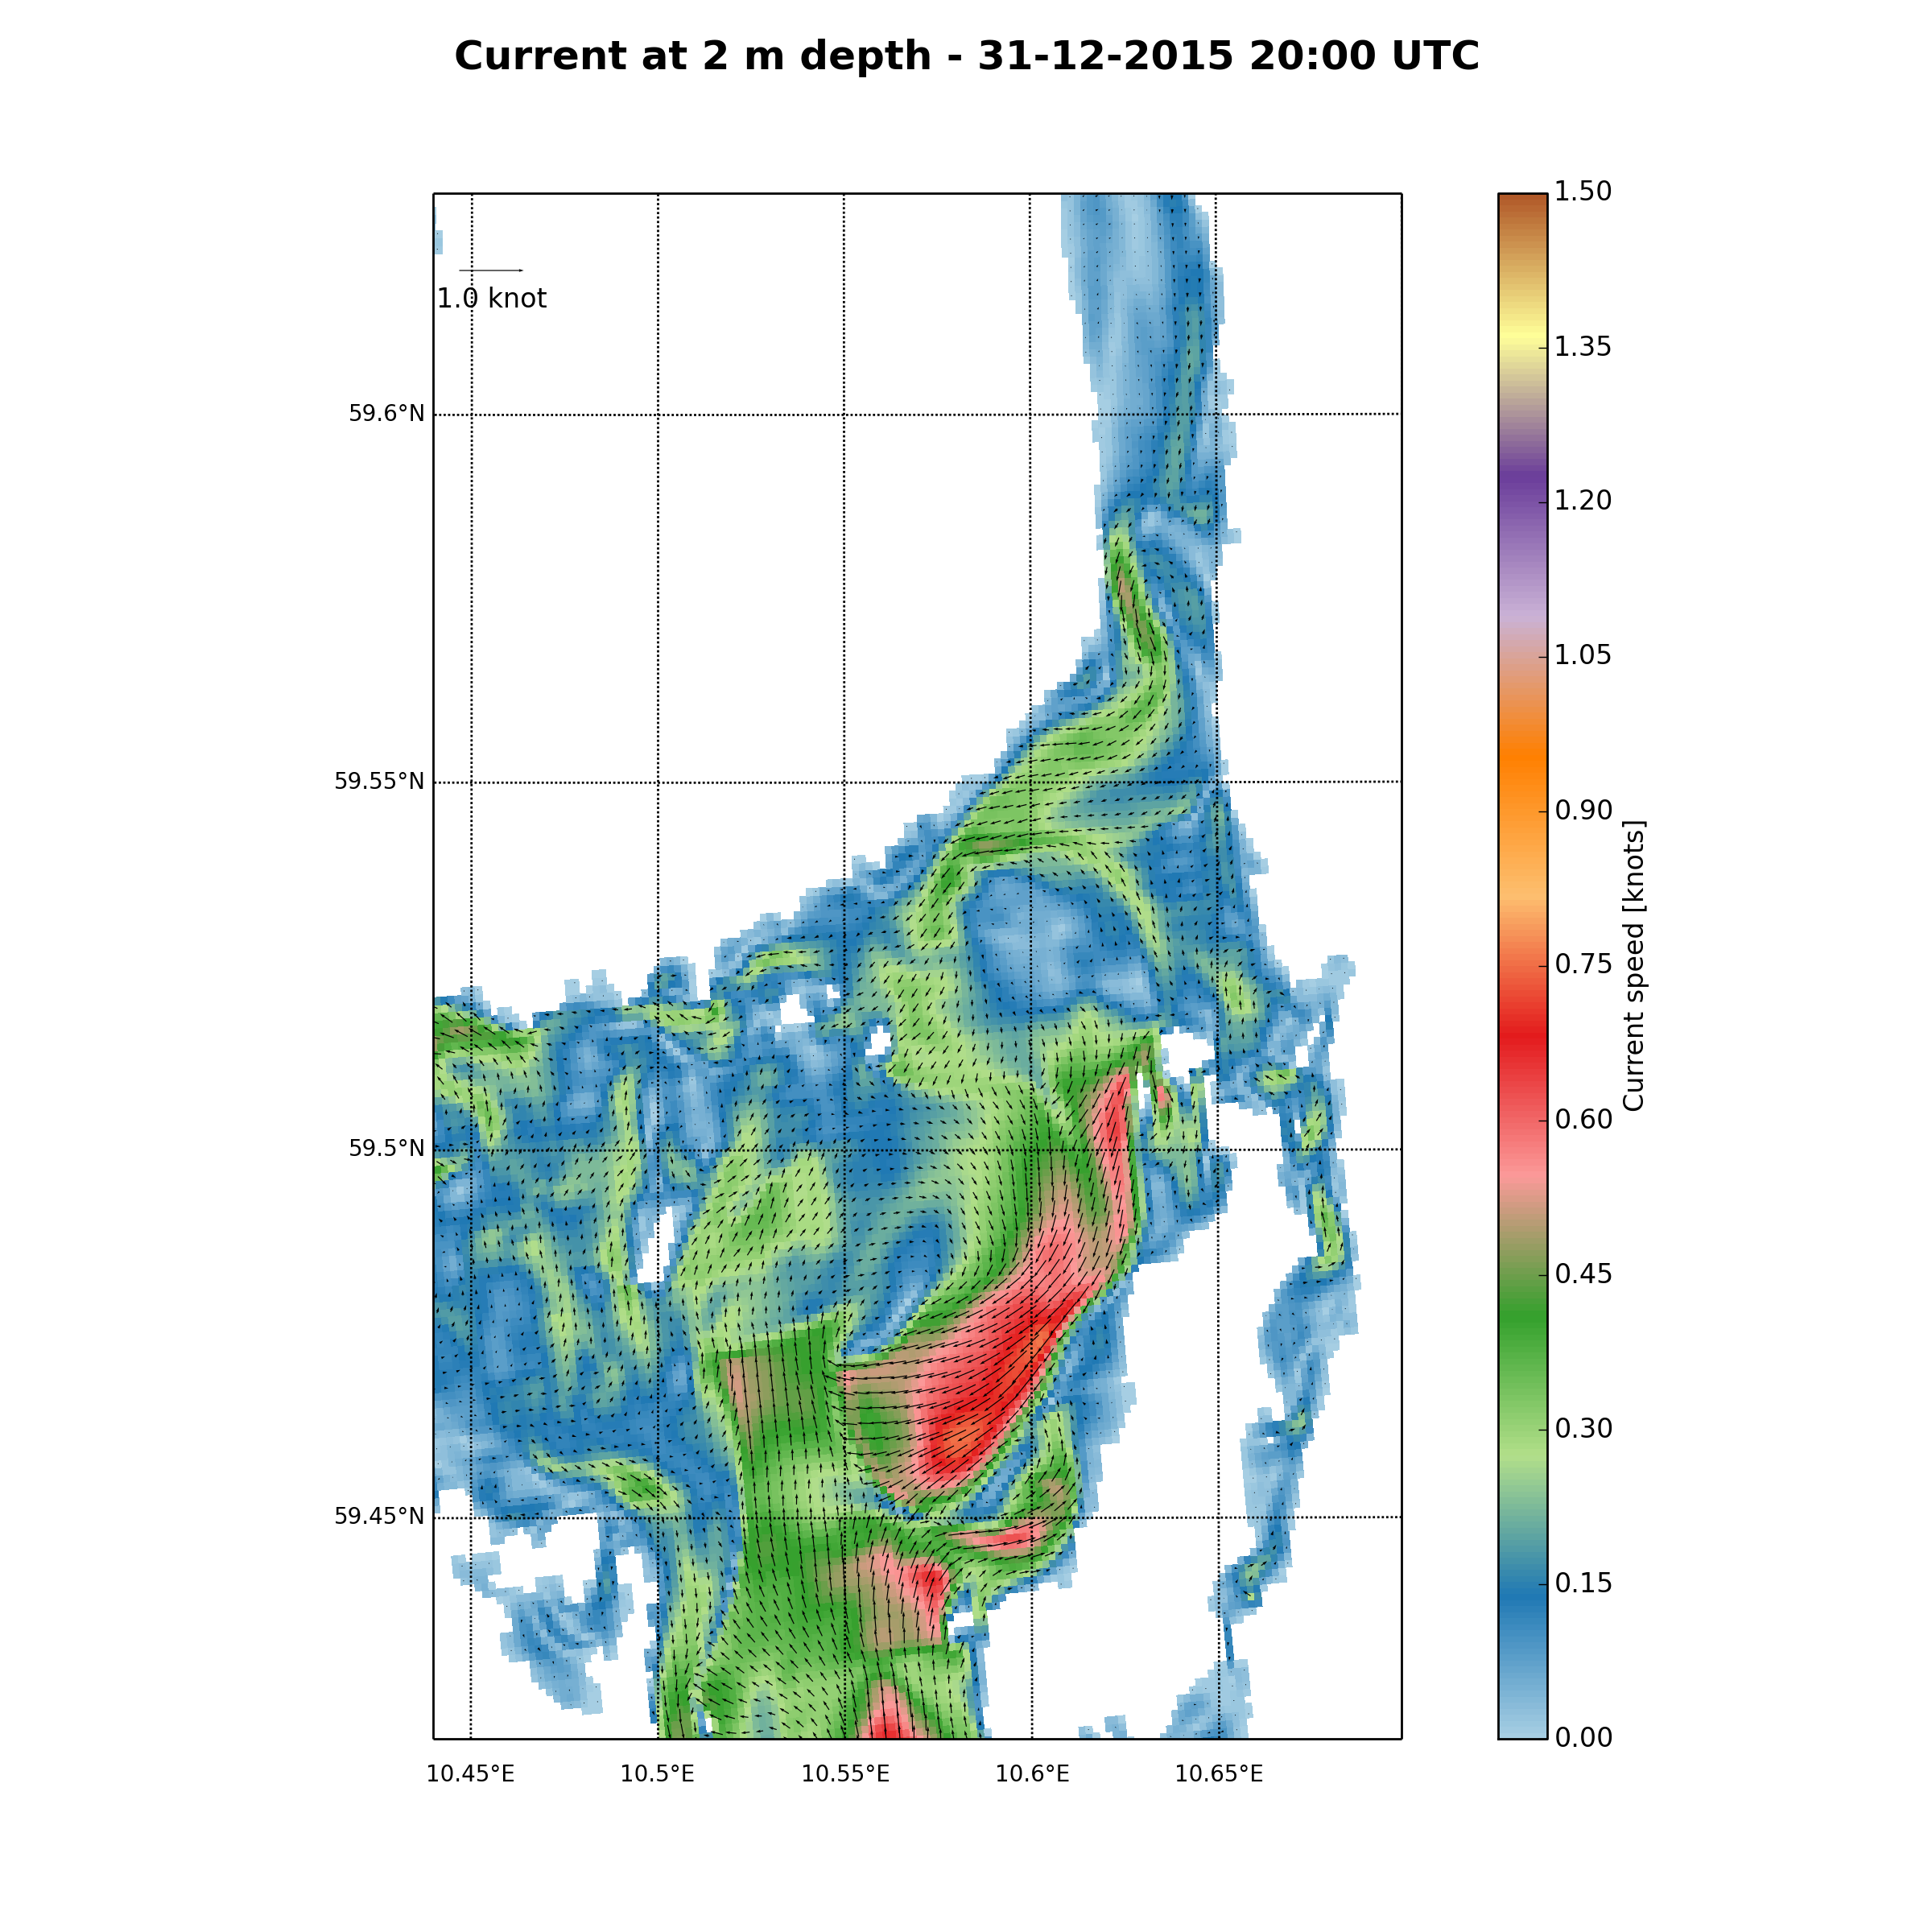
\includegraphics[height=8.5cm]{breidangen__56_current}}
   \rput[bl](0,7){\large \textbf{a)}}
   \rput[bl](7.5,7){\large \textbf{b)}}
   \rput[br](15,7){\large \textbf{c)}}
  \end{pspicture}
  \caption{\small a) The irregular coastline geometry and topography in the a) F{\ae}rder National Park and b) the Hvaler National Park. The grayscale in color bars indicates depth in meters. Note the many islands, narrow straits and channels present in these areas of the Oslofjord.}
  \label{fig:forecast_1}
 \end{center}
\end{figure}

